\documentclass[lecture.tex]{subfiles}

\begin{document}

\exercice{}
\video{https://youtu.be/iPdf8gAQtBE}
\enonce{rdm-0037}{}

Tracer le diagramme de $N$ et $\sigma_{xx}$ tout au long de la barre.

\begin{center}
  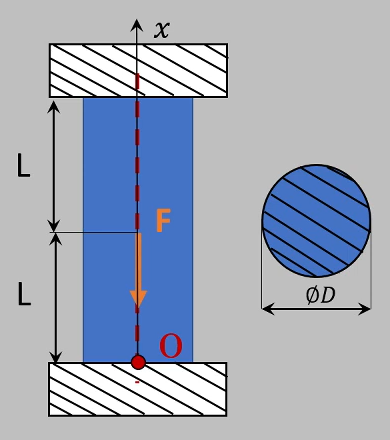
\includegraphics[scale=0.5]{figA0037.png}
\end{center}

Données d'entrée :

\begin{itemize}[label = \ding{110}, font = \tiny]
  \item 2L : Longueur de la barre (mm)
  \item D : Diamètre de la section transversale circulaire(mm)
  \item E : Module d'élasticité (Mpa)
  \item F : Force ponctuelle (N)
  \item $\rho$ : densité (Kg/$m^{3}$)
  \item g : gravité ($m / s^2$)
\end{itemize}


\finenonce{rdm-0037}
\finexercice


\end{document}
